\textbf{See the instruction for questions \inteval{\value{question}+1} to \inteval{\value{question}+2}.}

\begin{figure}[H]
    \centering
    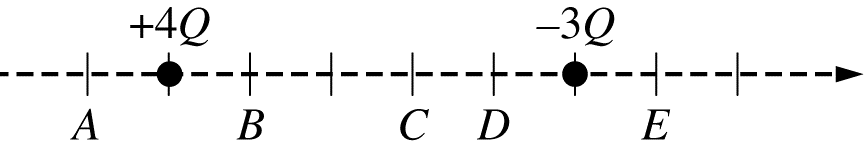
\includegraphics[scale=0.3]{images/img-013-021.png}
\end{figure}

Two small spheres are arranged along a line and carry charges of $+4 Q$ and $-3 Q$, as shown in the figure above. The vertical lines are equally spaced.

% Multiple Choice Question 29
\begin{questions}\setcounter{question}{28}\question
At which of the labeled points does the electric field point toward the right with the smallest magnitude?

\begin{oneparchoices}
\choice $A$
\choice $B$
\choice $C$
\choice $D$
\choice $E$
\end{oneparchoices}\end{questions}

% Multiple Choice Question 30
\begin{questions}\setcounter{question}{29}\question
At which of the labeled points does the electric potential have the largest positive value?

\begin{oneparchoices}
\choice $A$
\choice $B$
\choice $C$
\choice $D$
\choice $E$
\end{oneparchoices}\end{questions}

